% !TEX program = xelatex
\documentclass[oneside]{memoir}

\title{Notite examen - Probabilitati si Statistica}
\date{}
\author{Dinu Florin-Silviu \\ grupa 231}

\newcommand{\prim}{^\ensuremath{\prime}}
\newcommand{\secund}{^{\ensuremath{\prime\prime}}}

% \makeatletter
% \renewcommand{\@seccntformat}[1]{}
% \makeatother

\newenvironment{textColor}[1]{%
    \leavevmode\color{#1}\ignorespaces%
}{%
}%


\usepackage{tikz}
\usepackage{forest}
\usepackage{hyperref}
\usepackage{amsthm}
\usepackage{amssymb}
\usepackage[romanian]{babel}
\usepackage[a4paper, margin=3cm]{geometry}
\usepackage{enumitem}
\usepackage{listings}
\usepackage{fontspec}
\usepackage{xcolor}
\usepackage{textcomp}
\usepackage{graphicx}
\usepackage{tabularx}
\usepackage{pgfgantt}
\usepackage{titlesec}
\usepackage{mathtools}
\usepackage{diagbox}
\usepackage{pdfpages}
\usepackage{derivative}

\renewcommand{\printtoctitle}[1]{}

\NewEnviron{myequation*}{%
    \begin{equation*}
        % \begin{split}
    \scalebox{1.3}{$\BODY$}
        % \end{split}
    \end{equation*}
    }


\titleformat{\chapter}[display]
  {\normalfont\bfseries}{}{0pt}{\Huge}

\graphicspath{ {./img/} }

\newfontfamily{\ttconsolas}{Consolas}
\lstset{
%  tabsize=4,
extendedchars=true,
        basicstyle=\ttconsolas,
        % %upquote=false,
        % aboveskip=\baselineskip,
        columns=fixed,
        showstringspaces=false,
        extendedchars=true,
        breaklines=true,
        % prebreak = \raisebox{0ex}[0ex][0ex]{\ensuremath{\hookleftarrow}},
        showtabs=false,
        showspaces=false,
        identifierstyle=\ttfamily,
        % keywordstyle=\color[rgb]{0,0,1},
        % commentstyle=\color[rgb]{0.133,0.545,0.133},
        % stringstyle=\color[rgb]{0.627,0.126,0.941},
        % language=SQL
        frame=lines,
        literate=%
    {€}{\euro}1%
    {§}{\S}1%
    {°}{\textdegree{}}1%
    {ä}{{\"a}}1%
    {ö}{{\"o}}1%
    {ü}{{\"u}}1%
    {ß}{{\ss}}1%
    {Ä}{{\"A}}1%
    {Ö}{{\"O}}1%
    {Ü}{{\"U}}1%
    {µ}{\textmu}1%
    {¹}{{\textsuperscript{1}}}1%
    {²}{{\textsuperscript{2}}}1%
    {³}{{\textsuperscript{3}}}1%
    {¼}{\textonequarter}1%
    {½}{\textonehalf}1%
    {¢}{\textcent}1%
}


\tikzstyle{red state}=[
        draw = red,
        thick,
        fill = white,
        minimum size = 4mm,
        circle
    ]

\tikzstyle{blue state}=[
    draw = blue,
    thick,
    fill = white,
    minimum size = 4mm,
    circle
]

\tikzstyle{green state}=[
    draw = green,
    thick,
    fill = white,
    minimum size = 4mm,
    circle
]

\tikzset{
  gray box/.style={
    fill=gray!20,
    draw=gray,
    minimum width={1.2*#1ex},
    minimum height={1.5em},
  },
  annotation/.style={
    anchor=north,
  },
  level distance = 2cm
}

\newtheorem*{theorem}{Teorema}
\renewcommand\qedsymbol{QED}

\begin{document}
\pagenumbering{gobble}
\maketitle
\tableofcontents

\newpage
\pagenumbering{arabic}

\chapter[Probabilitati]{Probabilitati}
\section[Evenimente independente]{Evenimente independente}
\paragraph*{Exemplu} Se considera 2 urne $U_1(3a, 5n)$ si $U_2(4a, 6n)$. Din fiecare se extrage o bila. Care este probabilitatea ca bila sa fie alba?
\subparagraph*{Solutie} Notam
\begin{enumerate}
    \item A = extragem din $U_1$ o bila alba
    \item B = extragem din $U_2$ o bila alba
\end{enumerate}
\subparagraph*{Calculam} $P(A\cup B)$
\begin{center}
    \begin{myequation*}
\mathbf{P(A\cup B) = P(A) + P(B) - P(A\cap B)} = \frac{3}{8} + \frac{4}{10} - \frac{3}{8}*\frac{4}{10} = \frac{5}{8}
    \end{myequation*}
\end{center}

\section[Schema bilei nerevenite]{Schema bilei nerevenite}
\begin{center}
    \begin{myequation*}
        P_n(k) = \frac{C^k_a \cdot  C^{n-k}_b}{C^n_{a+b}}
    \end{myequation*}
\end{center}
\paragraph*{Exemplu} Intr-o bila se afla 5 bile rosii, 6 albe si 7 negre. Se extrag simultan din urna 4 bile.
\begin{enumerate}
    \item Care e probabilitatea ca toate bilele sa fie rosii?
    \item Toate sa fie albe?
    \item Nicio bila sa nu fie rosie?
    \item O bila sa fie rosie si una alba?
    \item Cel putin 2 bile sa fie rosii?
\end{enumerate}

\subparagraph*{Solutie}
\subparagraph*{1.}
\begin{center}
    \begin{myequation*}
P_{18}(4) = \frac{C^4_5 \cdot  C^0_{13}}{C^4_{18}}
    \end{myequation*}
\end{center}

\subparagraph*{2.}
\begin{center}
    \begin{myequation*}
P_{18}(4) = \frac{C^4_6 \cdot  C^0_{13}}{C^4_{18}}
    \end{myequation*}
\end{center}

\subparagraph*{3.}
\begin{center}
    \begin{myequation*}
P_{18}(4) = \frac{C^4_{13} \cdot  C^0_{13}}{C^4_{18}}
    \end{myequation*}
\end{center}

\subparagraph*{4.}
\begin{center}
    \begin{myequation*}
P = \frac{C^5_{1} \cdot  C^6_{1} \cdot  C^2_7}{C^4_{18}}
    \end{myequation*}
\end{center}

\subparagraph*{5.}
\begin{center}
    \begin{myequation*}
P = \frac{C^5_{2} \cdot  C^2_{13} + C_5^3\cdot C_{13}^1\cdot C_5^4}{C^4_{18}}
    \end{myequation*}
\end{center}

\section[Schema bilei revenite]{Schema bilei revenite}
\begin{center}
    \begin{myequation*}
P_n(k) = C_n^k \cdot  p^k\cdot  (1-p)^{n-k}
    \end{myequation*}
\end{center}

\paragraph*{Exemplu} Aruncam o moneda de 3 ori. Care e probabilitatea a 3 aversuri?
\subparagraph*{Solutie}
\begin{center}
    \begin{myequation*}
P_3(3) = C_3^3 \cdot  (\frac{1}{2})^3 \cdot  (1-\frac{1}{2})^{0} = \frac{1}{8}
    \end{myequation*}
\end{center}

\section[Probabilitati conditionate]{Probabilitati conditionate}
\begin{center}
    \begin{myequation*}
P(A/B) = \frac{P(A\cap B)}{P(B)}
    \end{myequation*}
\end{center}

\paragraph*{Exemplu} Aruncam o moneda de 3 ori. Care este probabilitatea a 3 aversuri stiind ca prima aruncare a fost un avers?

\subparagraph*{Solutie} Fie A = 3 aversuri si B = prima a fost avers
\begin{center}
    \begin{myequation*}
P(A/B) = \frac{P(A \cap B)}{P(B)} = \frac{\frac{1}{8}}{\frac{1}{2}}
    \end{myequation*}
\end{center}

\paragraph*{Exemplul 2} Se arunca succesiv 2 zaruri. A = primul zar obtinem cel mult 3 puncte si B = suma cifrelor sa fie 8. Calculati: P(A), P(B), P(B/A), P(A/B).
\subparagraph*{Solutie}

\begin{center}
    \begin{myequation*}
P(A) = \frac{3}{6} = \frac{1}{2}
    \end{myequation*}
\end{center}
\begin{center}
    \begin{myequation*}
P(B) = \frac{5}{36}
    \end{myequation*}
\end{center}
\begin{center}
    \begin{myequation*}
P(B/A) = \frac{P(B\cap A)}{P(A)} = \frac{\frac{1}{18}}{\frac{5}{36}} = \frac{2}{5}
    \end{myequation*}
\end{center}

\section[Formula probabilitatii totale]{Formula probabilitatii totale}
Fie spatiul $\Omega$ impartit in 3 evenimente disjuncte 2 cate 2: $B_1$, $B_2$, $B_3$. Pentru orice eveniment A:
\begin{center}
    \begin{equation*}
        \begin{split}
P(A) &= P(A\cap B_1) +  P(A\cap B_2) +  P(A\cap B_3) = \\ 
&= P(A/B_1) \cdot  P(B_1) + P(A/B_2) \cdot  P(B_2) + P(A/B_3) \cdot  P(B_3)
        \end{split}
    \end{equation*}
\end{center}

\section[Bayes]{Bayes}
\begin{center}
    \begin{myequation*}
        P(B/A) = \frac{P(A/B) \cdot  P(B)}{P(A)}
    \end{myequation*}
\end{center}

\paragraph*{Exemplu} Intr-un depozit sunt aduse piese de acelasi fel fabricate in 2 ateliere, primul are 3 masini si produce in proportie de 99\% piese corespunzatoare si de 1\% defecte. Al doilea are 2 masini si produce 98\% corespunzatoare si 2\% defecte.
\begin{enumerate}
    \item Care este probabilitatea ca o piesa luata aleatoriu din depozit sa fie corespunzatoare
    \item Daca se ia la intamplare o piesa corespunzatoare, cu ce probabilitatea provine de la primul atelier?
\end{enumerate}

\subparagraph*{Solutie} Notam $B_1$ = piesa de la atelierul 1, $B_2$ = piesa de la atelierul 2 si $A$ = piesa corespunzatoare

\subparagraph*{1. Metoda 1:} $P(B_1)= \frac{3}{5}$ si $P(B_2) = \frac{2}{5}$
\begin{center}
    \begin{equation*}
        \begin{split}
P(A) &= P(A/B_1)\cdot P(B_1) + P(A/B_2) \cdot  P(B_2) \\
&= \frac{99}{100}\cdot \frac{3}{5} + \frac{98}{100}\cdot \frac{2}{5} = \frac{493}{500}
        \end{split}
    \end{equation*}
\end{center}
\subparagraph*{1. Metoda 2:}
\begin{center}
    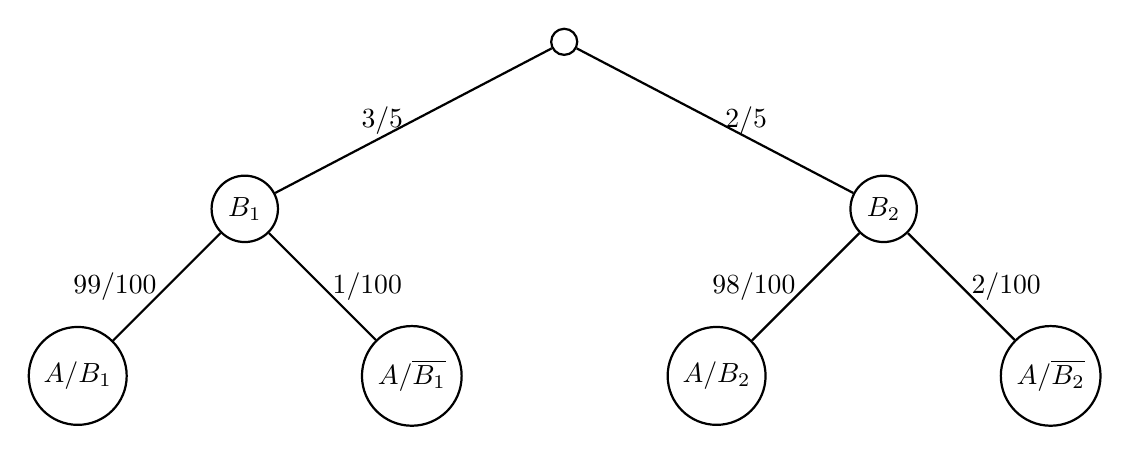
\begin{tikzpicture}[node distance={30mm}, thick, main/.style = {draw, circle} ]
        \node[main] (0) {};
        \node[main] (B1) [below left of = 0, left = 1.5cm] {$B_1$};
        \node[main] (B2) [below right of = 0, right = 1.5cm] {$B_2$};
        \node[main] (AB1) [below left of = B1]{$A/B_1$};
        \node[main] (nAB1) [below right of = B1]{$A/\overline{B_1}$};
        \node[main] (AB2) [below left of = B2]{$A/B_2$};
        \node[main] (nAB2) [below right of = B2]{$A/\overline{B_2}$};


        \draw[-] (0) -- (B1) node [midway,left] {3/5};
        \draw[-] (0) -- (B2) node [midway, right] {2/5};
        \draw[-] (B1) -- (AB1) node [midway, left] {99/100};
        \draw[-] (B1) -- (nAB1) node [midway, right] {1/100};
        \draw[-] (B2) -- (AB2) node [midway, left] {98/100};
        \draw[-] (B2) -- (nAB2) node [midway, right] {2/100};

    \end{tikzpicture}
\end{center}

\begin{center}
    \begin{equation*}
P(A) = \frac{3}{5} \cdot  \frac{99}{100} + \frac{2}{5} \cdot  \frac{98}{100} = \frac{493}{500}
    \end{equation*}
\end{center}

\subparagraph*{2.}
\begin{center}
    \begin{equation*}
        \begin{split}
P(B_1/A) &= \frac{P(A/B_1) \cdot  P(B_1)}{P(A)}\\
&=\frac{\frac{99}{100} \cdot  \frac{3}{5}}{\frac{493}{500}} = \frac{99}{493}
        \end{split}
    \end{equation*}
\end{center}

\paragraph*{Exemplul 2.} Se considera 2 urne avand $U_1(6a,4n)$ si $U_2(5a,10n)$. Se arunca un zar si daca se obtine un numar impar, se scoate 1 bila din prima urna, iar daca se obtine numar par, se scoate 1 bila din a doua urna.
\begin{enumerate}
    \item Care este probabilitatea de a obtine o bila alba?
    \item Se extrage 1 bila alba. Care e probabilitatea sa fie din $U_1$?
\end{enumerate}

\subparagraph*{Solutie} Notam $B_1$ = nr impar si $B_2$ = nr par si $A$ = bila extrasa este alba.

\subparagraph*{1. Metoda 1:}
\begin{center}
    \begin{equation*}
        \begin{split}
P(A) &= P(A/B_1) \cdot  P(B_1) + P(A/B_2) \cdot  P(B_2) \\ 
&=\frac{6}{10}\cdot \frac{1}{2}+ \frac{5}{15}\cdot \frac{1}{2} = \frac{7}{15}
        \end{split}
    \end{equation*}
\end{center}

\subparagraph*{1. Metoda 2:}
\begin{center}
    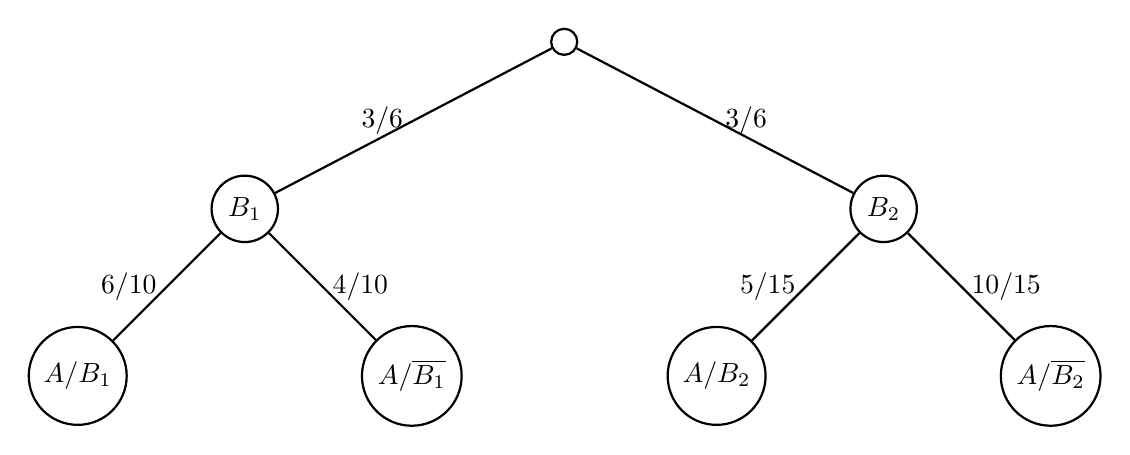
\begin{tikzpicture}[node distance={30mm}, thick, main/.style = {draw, circle} ]
        \node[main] (0) {};
        \node[main] (B1) [below left of = 0, left = 1.5cm] {$B_1$};
        \node[main] (B2) [below right of = 0, right = 1.5cm] {$B_2$};
        \node[main] (AB1) [below left of = B1]{$A/B_1$};
        \node[main] (nAB1) [below right of = B1]{$A/\overline{B_1}$};
        \node[main] (AB2) [below left of = B2]{$A/B_2$};
        \node[main] (nAB2) [below right of = B2]{$A/\overline{B_2}$};


        \draw[-] (0) -- (B1) node [midway,left] {3/6};
        \draw[-] (0) -- (B2) node [midway, right] {3/6};
        \draw[-] (B1) -- (AB1) node [midway, left] {6/10};
        \draw[-] (B1) -- (nAB1) node [midway, right] {4/10};
        \draw[-] (B2) -- (AB2) node [midway, left] {5/15};
        \draw[-] (B2) -- (nAB2) node [midway, right] {10/15};

    \end{tikzpicture}
\end{center}

\subparagraph*{2.}
\begin{center}
    \begin{equation*}
        \begin{split}
P(B_1/A) &= \frac{P(A/B_1) \cdot  P(B_1)}{P(A)}\\
&=\frac{\frac{6}{10}\cdot \frac{1}{2}}{\frac{7}{15}} = \frac{9}{14}
        \end{split}
    \end{equation*}
\end{center}

\section[Variabile aleatoare discrete]{Variabile aleatoare discrete unidimensionale}
\subsection*{Definitii}
Fie
\begin{center}
    \begin{equation*}
X \sim \begin{bmatrix}
    x_1 & x_2 & \dots & x_n \\
    p_1 & p_2 & \dots & p_n
\end{bmatrix}
    \end{equation*}
\end{center}
\begin{center}
    \begin{equation*}
Y \sim \begin{bmatrix}
    y_1 & y_2 & \dots & y_n \\
    q_1 & q_2 & \dots & q_n
\end{bmatrix}
    \end{equation*}
\end{center}

\paragraph*{Functia de repartitie (cdf)} $F:\mathbb{R}\rightarrow[0,1]$, $F(X) = P(X\leq x)$

\begin{center}
    \begin{equation*}
        \begin{split}
F(x) = \left\{
    \begin{array}{ll}
          0, x \leq x_1 \\
        0 + p_1, x \in (x_1, x_2]\\
          0 + p_1 + p_2, x \in (x_2, x_3] \\
          \cdots \\
          \sum_{i=1}^{n}p_i, x \in (x_{n-1}, x_n] \\
          1, x \in (x_n, \infty)
    \end{array} 
    \right. 
        \end{split}
    \end{equation*}
\end{center}

\subsection*{Aritmetica}
\begin{center}
    \begin{equation*}
X + Y \sim \begin{bmatrix}
    x_i+y_j \\
    p_{ij}
\end{bmatrix}
    \end{equation*}
\end{center}

\begin{center}
    \begin{equation*}
X \cdot  Y \sim \begin{bmatrix}
    x_i\cdot y_j \\
    p_{ij}
\end{bmatrix}
    \end{equation*}
\end{center}

\begin{center}
    \begin{equation*}
\frac{X}{Y} \sim \begin{bmatrix}
    \frac{x_i}{y_j} \\
    p_{ij}
\end{bmatrix}
    \end{equation*}
\end{center}

\begin{center}
    \begin{equation*}
a + X \sim \begin{bmatrix}
    x_i + a \\
    p_{i}
\end{bmatrix}
    \end{equation*}
\end{center}

\begin{center}
    \begin{equation*}
a \cdot  X \sim \begin{bmatrix}
    x_i\cdot  a \\
    p_{i}
\end{bmatrix}
    \end{equation*}
\end{center}

\begin{center}
    \begin{equation*}
X^n \sim \begin{bmatrix}
    x_i^n \\
    p_{i}
\end{bmatrix}
    \end{equation*}
\end{center}

\subsection*{Media}
\begin{center}
    \begin{equation*}
E(X) = \sum_{i=1}^{n}x_i*p_i
    \end{equation*}
\end{center}

\begin{center}
    \begin{equation*}
E(X+Y) = E(X) + E(Y)
    \end{equation*}
\end{center}

\begin{center}
    \begin{equation*}
E(cX) = c\cdot E(X)
    \end{equation*}
\end{center}

\begin{center}
    \begin{equation*}
E(c) = c
    \end{equation*}
\end{center}

\subsection*{Dispersia}
\begin{center}
    \begin{equation*}
Var(X) = E(X^2) - E^2(X)
    \end{equation*}
\end{center}

\begin{center}
    \begin{equation*}
Var(aX) = a^2\cdot Var(X)
    \end{equation*}
\end{center}

\begin{center}
    \begin{equation*}
Var(X+Y) = Var(X) + Var(Y) - cov(X,Y)
    \end{equation*}
\end{center}

\subsection*{Deviatia standard}
\begin{center}
    \begin{equation*}
\sigma = \sqrt{Var(X)}
    \end{equation*}
\end{center}


\subsection*{Covarianta}
\begin{center}
    \begin{equation*}
cov(X,Y) = E(X\cdot Y) - E(X) \cdot E(Y)
    \end{equation*}
\end{center}
\paragraph*{cov(X,Y) = 0} $\rightarrow$ necorelate
\paragraph*{X, Y independente} $\rightarrow$ cov(X,Y) = 0 (inversa nu e valabila)


\section[Variabile discrete bidimensionale]{Variabile discrete bidimensionale}

\subsection*{Definitii}
\begin{center}
    \begin{tabularx}{0.8\textwidth} {
            | >{\centering\arraybackslash}X
            || >{\centering\arraybackslash}X
             >{\centering\arraybackslash}X
             >{\centering\arraybackslash}X
             >{\centering\arraybackslash}X
            || >{\centering\arraybackslash}X
            |}
        \hline
        \backslashbox{x}{y} &  $y_1$ & $y_2$ & $\dots$ & $y_n$ & $p_i$ \\
        \hline
        $x_1$ & $p_{11}$ & $p_{12}$ & $\dots$ & $p_{1n}$ & $p_1$     \\    
        $x_2$ & $p_{21}$ & $p_{22}$ & $\dots$ & $p_{2n}$ & $p_n$     \\                      
        $\cdots$  & $\cdots$ & $\cdots$& $\cdots$& $\cdots$& $\cdots$  \\     
        $x_m$ & $p_{m1}$ & $p_{m2}$ & $\dots$ & $p_{mn}$ & $p_m$     \\   
        \hline
        $q_j$ & $q_1$ & $q_2$ & $\dots$ & $q_n$ & 1 \\
        \hline
    \end{tabularx}
\end{center}

\begin{center}
    \begin{equation*}
X \sim \begin{bmatrix}
    x_1 & x_2 & \dots & x_n \\
    p_1 & p_2 & \dots & p_n
\end{bmatrix}
    \end{equation*}
\end{center}
\begin{center}
    \begin{equation*}
Y \sim \begin{bmatrix}
    y_1 & y_2 & \dots & y_n \\
    q_1 & q_2 & \dots & q_n
\end{bmatrix}
    \end{equation*}
\end{center}

\subsection*{Covarianta}
\begin{center}
    \begin{equation*}
cov(X,Y) = E(X\cdot Y) - E(X) \cdot E(Y)
    \end{equation*}
\end{center}
\paragraph*{cov(X,Y) = 0} $\rightarrow$ necorelate
\paragraph*{X, Y independente} $\rightarrow$ cov(X,Y) = 0 (inversa nu e valabila)

\subsection*{Coeficientul de corelatie}
\begin{center}
    \begin{equation*}
\rho_{X,Y} = \frac{cov(X,Y)}{\sqrt[]{Var(X)} \cdot \sqrt[]{Var(Y)}} = \frac{E(X\cdot Y) - E(X) \cdot E(Y)}{\sqrt[]{Var(X)} \cdot \sqrt[]{Var(Y)}}
    \end{equation*}
\end{center}


\subsection*{Verificare dependenta}
Verificam daca $P(X=x, Y=y) = P(X=x) \cdot P(Y=y)$

\section[Variabile continue unidimensionale]{Variabile continue unidimensionale}
\subsection*{Definitie}
Fie X variabila aleatoare avand functia de repartitie (cdf) F. X este de tip continuu daca $F(x) = \int_{-\infty}^{x}f(t) dt, \forall x \in \mathbb{R}$

\subsection*{Densitatea de repartitie - pmf} Densitatea de repartitie (\textbf{pmf}) este $f:\mathbb{R}\rightarrow \mathbb{R}$ cu proprietatile:
\begin{enumerate}
    \item $f(x) \geq 0$
    \item $\int_{-\infty}^{\infty}f(x)dx = 1$
\end{enumerate}

\paragraph*{Observatie:} 
\begin{center}
    \begin{equation*}
        \begin{split}
&P(X\le a) = P(X\leq a) = F(a) = \int_{-\infty}^{a}f(x)dx\\
&P(X > a) = 1 - P(X \leq a)\\
&P(a \leq X \leq b) = P(X \leq b) - P(X \leq a)
        \end{split}
    \end{equation*}
\end{center}

\subsection*{Media}
\begin{center}
    \begin{equation*}
E(X) = \int_{-\infty}^{\infty}x\cdot f(x) dx
    \end{equation*}
\end{center}

\subsection*{Dispersia}
\begin{center}
    \begin{equation*}
Var(X) = E(X^2) - E^2(X)
    \end{equation*}
\end{center}
Unde
\begin{center}
    \begin{equation*}
E(X^2) = \int_{-\infty}^{\infty}x^2\cdot f(x) dx
    \end{equation*}
\end{center}

\subsection*{Deviatia standard}
\begin{center}
    \begin{equation*}
\sigma = \sqrt{Var(X)}
    \end{equation*}
\end{center}

\section[Variabile continue bidimensionale]{Variabile continue bidimensionale}
\subsection*{Definitie}
La fel ca la unidimensionale, doar cu 2 variabile

\subsection*{Densitatea de repartitie - pmf} Densitatea de repartitie (\textbf{pmf}) este $f:\mathbb{R}x\mathbb{R}\rightarrow \mathbb{R}$ cu proprietatile:
\begin{enumerate}
    \item $f(x,y) \geq 0$
    \item $\int_{-\infty}^{\infty}\int_{-\infty}^{\infty}f(x,y)dx dy = 1$
\end{enumerate}

\subsection*{Repartitiile marginale}
\begin{center}
    \begin{equation*}
        \begin{split}            
&f_{\mathbf{x}}(\mathbf{x}) = \int_{-\infty}^{\infty}f(x,y) \mathbf{dy}\\
&f_{\mathbf{y}}(\mathbf{y}) = \int_{-\infty}^{\infty}f(x,y) \mathbf{dx}
    \end{split}
    \end{equation*}
\end{center}

\subsection*{Independenta}
\begin{center}
    \begin{equation*}
f(x,y) = f_x(x) \cdot f_y(y)
    \end{equation*}
\end{center}

\subsection*{Media}
\begin{center}
    \begin{equation*}
        \begin{split}
&E(X) = \int_{-\infty}^{\infty} x \cdot f_x(x) dx \\
&E(Y) = \int_{-\infty}^{\infty} x \cdot f_y(y) dy \\
&E(X\cdot Y) = \int_{-\infty}^{\infty} \int_{-\infty}^{\infty} x\cdot y \cdot f(x,y) dy dx
        \end{split}
    \end{equation*}
\end{center}

\subsection*{Dispersia}
\begin{center}
    \begin{equation*}
Var(X) = E(X^2) - E^2(X)
    \end{equation*}
\end{center}

\subsection*{Covarianta}
\begin{center}
    \begin{equation*}
cov(X,Y) = E(X\cdot Y) - E(X) \cdot E(Y)
    \end{equation*}
\end{center}
\paragraph*{cov(X,Y) = 0} $\rightarrow$ necorelate
\paragraph*{X, Y independente} $\rightarrow$ cov(X,Y) = 0 (inversa nu e valabila)

\section[Repartitii clasice]{Repartitii clasice}
\subsection*{Normale}
\begin{center}
    \begin{myequation*}
f(x) = \frac{1}{\sigma \cdot \sqrt{2 \cdot \pi}} \cdot e^{- \frac{(x-\mu)^2}{2\sigma^2}}
    \end{myequation*}
\end{center}
\subsection*{Bernoulli}
\begin{center}
    \begin{equation*}
P_n(k) = C_n^k \cdot p^k \cdot (1-p)^{n-k}
    \end{equation*}
\end{center}
\subsection*{Geometrice}
\begin{center}
    \begin{equation*}
f(x) = 1- (1-p)^{x+1}
    \end{equation*}
\end{center}
\subsection*{Exponentiale}
\begin{center}
    \begin{myequation*}
f_{x_i}(x_i) = \lambda \cdot e^{-\lambda \cdot x_i}
    \end{myequation*}
\end{center}



\chapter[Statistica]{Statistica}

\section[Intervale de incredere]{Intervale de incredere}
\subsection*{Repartitia normala}
$N(\mu, \sigma)$
\begin{center}
    \begin{myequation*}
\overline{X} - Z_{\frac{\alpha}{2}} \cdot \frac{\sigma}{\sqrt{n}} \le \mu \le  \overline{X} + Z_{\frac{\alpha}{2}} \cdot \frac{\sigma}{\sqrt{n}}
    \end{myequation*}
\end{center}

\subsection*{Normal conservatoare}
\begin{center}
    \begin{myequation*}
\overline{X} - Z_{\frac{\alpha}{2}} \cdot \frac{1}{2\cdot\sqrt{n}} \le \mu \le  \overline{X} + Z_{\frac{\alpha}{2}} \cdot \frac{1}{2\cdot\sqrt{n}}
    \end{myequation*}
\end{center}

\subsection*{Regula degetului mare 95\%}
\begin{center}
    \begin{myequation*}
\overline{X} - \frac{1}{\sqrt{n}} \le \mu \le  \overline{X} + \frac{1}{\sqrt{n}}
    \end{myequation*}
\end{center}

\section[Actualizare Bayesiana]{Actualizare Bayesiana}
\begin{center}
    \begin{myequation*}
O(E) = \frac{P(E)}{P(\overline{E})}
    \end{myequation*}
\end{center}

\begin{center}
    \begin{myequation*}
O(M/F) = \frac{P(M/F)}{P(M/\overline{F})}
    \end{myequation*}
\end{center}

\section[Verosimilitate maxima (MLE)]{Verosimilitate maxima (MLE)}
\begin{center}
    \begin{myequation*}
\pdv{\ln p}{p} = 0
    \end{myequation*}
\end{center}




\chapter[Anexa 1 - Derivate si integrale]{Anexa 1 - Derivate si integrale}
\section[Functia $\Gamma$]{Functia $\Gamma$}
\begin{center}
    \begin{equation*}
        \begin{split}
&\Gamma(z) = \int_{0}^{\infty} t^{z-1}\cdot e^{-t}dt\\
&n\in \mathbb{N}\\
&\Gamma(n) = (n-1)!
        \end{split}
    \end{equation*}
\end{center}

\section[Functia B]{Functia B}

\begin{center}
    \begin{equation*}
        \begin{split}
&B(x,y) = \int_0^1 t^{x-1}\cdot (i-t)^{y-1}dt\\
&Re(x) > 0\ si \ Re(y) > 0\\
&B(x,y) = \frac{\Gamma(x)\cdot \Gamma(y)}{\Gamma(x+y)} = B(y,x)
        \end{split}
    \end{equation*}
\end{center}

\begin{center}
    \begin{equation*}
\int e^{\alpha\cdot x} = \frac{e^{\alpha\cdot x}}{\alpha} + C
    \end{equation*}
\end{center}

\section[Integralele Wallis]{Integralele Wallis}
\begin{center}
    \begin{equation*}
        \begin{split}
&W_n=\int_0^{\frac{\pi}{2}} sin^n \Theta d\Theta = \int_0^{\frac{\pi}{2}} cos^n \Theta d\Theta\\
&W_n = \frac{1}{2}\cdot B(\frac{n+1}{2},\frac{1}{2})
        \end{split}
    \end{equation*}
\end{center}

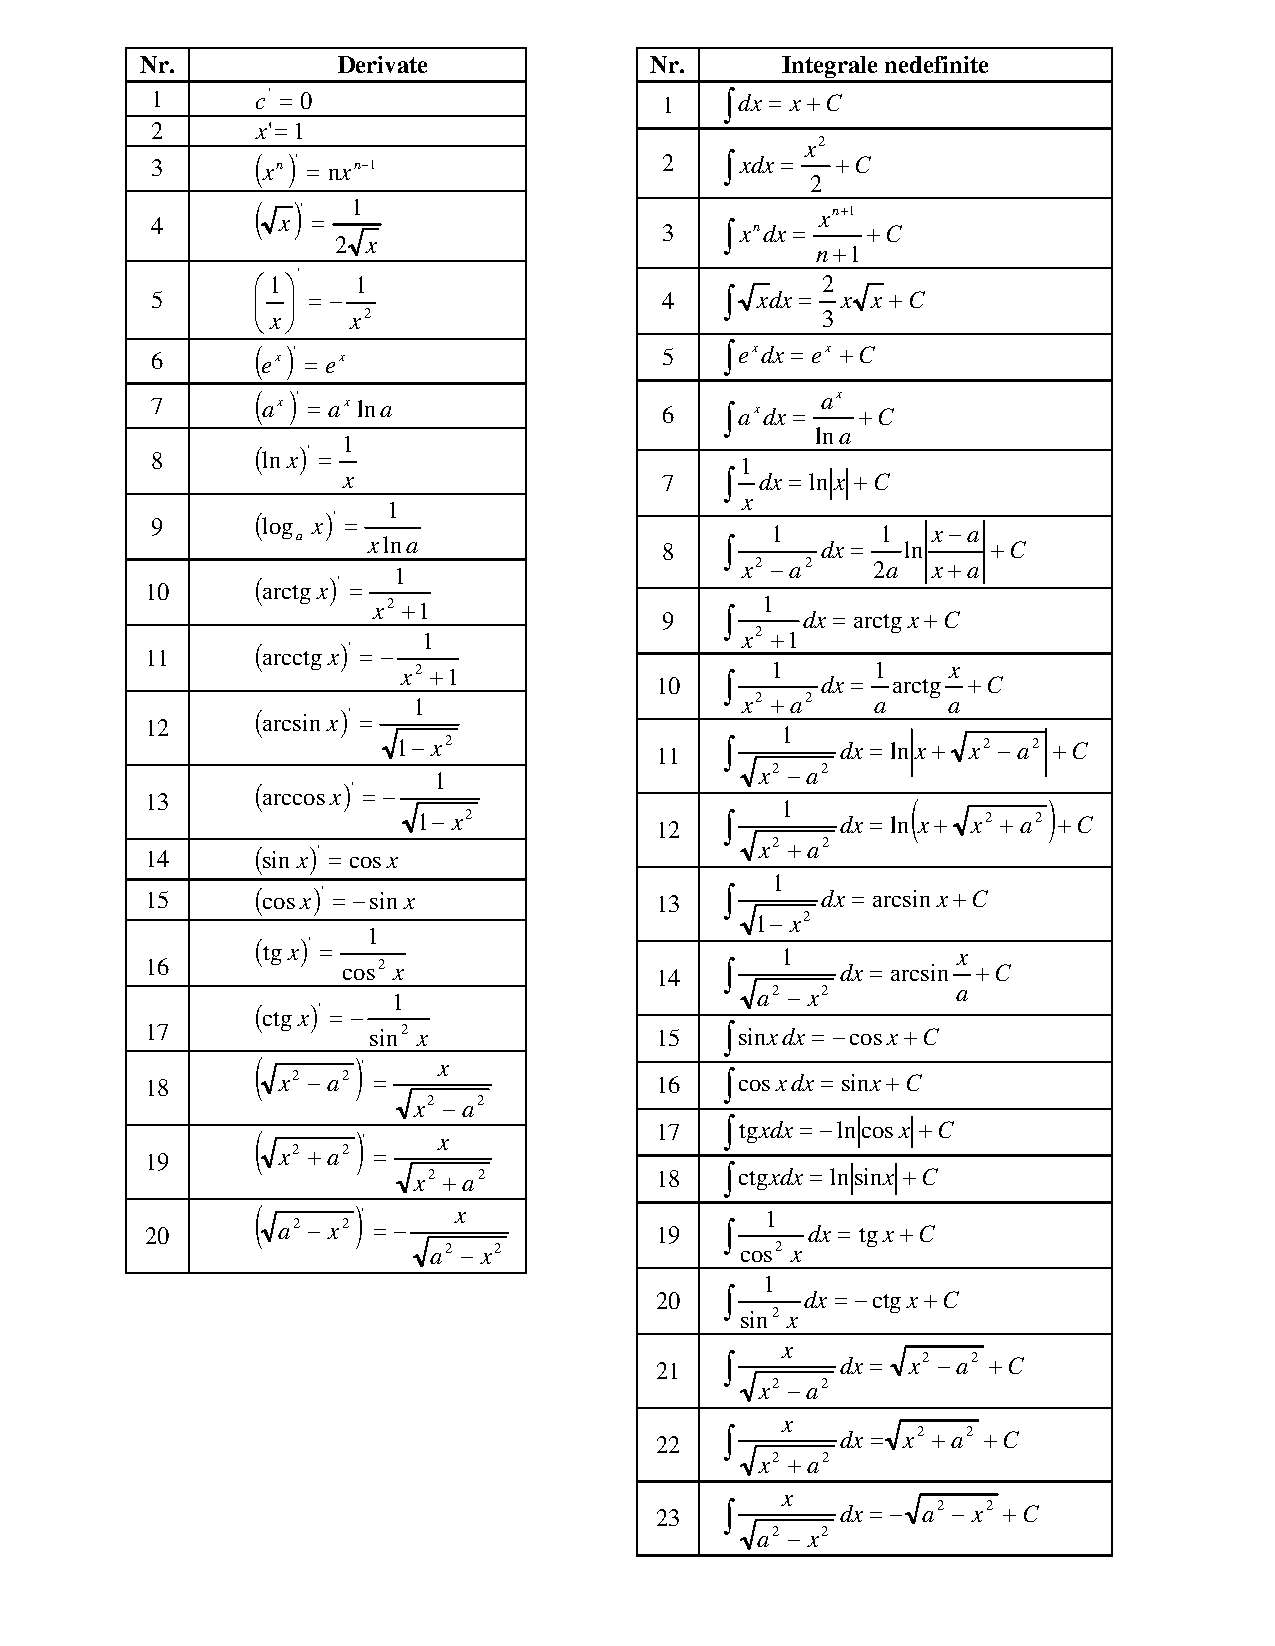
\includepdf[pages=-]{TABEL - Derivate si integrale.pdf}

\chapter[Anexa 2 - Functii trigonometrice]{Anexa 2 - Functii trigonometrice}
\begin{center}
    \begin{tabularx}{0.8\textwidth} {
            | >{\centering\arraybackslash}X
            || >{\centering\arraybackslash}X
            | >{\centering\arraybackslash}X
            | >{\centering\arraybackslash}X
            | >{\centering\arraybackslash}X
            | >{\centering\arraybackslash}X
            |}
        \hline
        x &  0 & $\frac{\pi}{6}$ & $\frac{\pi}{4}$ & $\frac{\pi}{3}$ & $\frac{\pi}{2}$ \\
        \hline
        \hline
        $\sin x$ & 0 & $\frac{1}{2}$ & $\frac{\sqrt{2}}{2}$ & $\frac{\sqrt{3}}{2}$ & 1 \\
        \hline
        $\cos x$ & 1 & $\frac{\sqrt{3}}{2}$ & $\frac{\sqrt{2}}{2}$ & $\frac{1}{2}$ & 0 \\
        \hline
        $ \tan x$ & 0 & $\frac{1}{\sqrt{3}}$ & 1 & $\sqrt{3}$ & / \\
        \hline
        $\cot x$ & / & $\sqrt{3}$ & 1 & $\frac{1}{\sqrt{3}}$ & 0 \\
        \hline
    \end{tabularx}
\end{center}
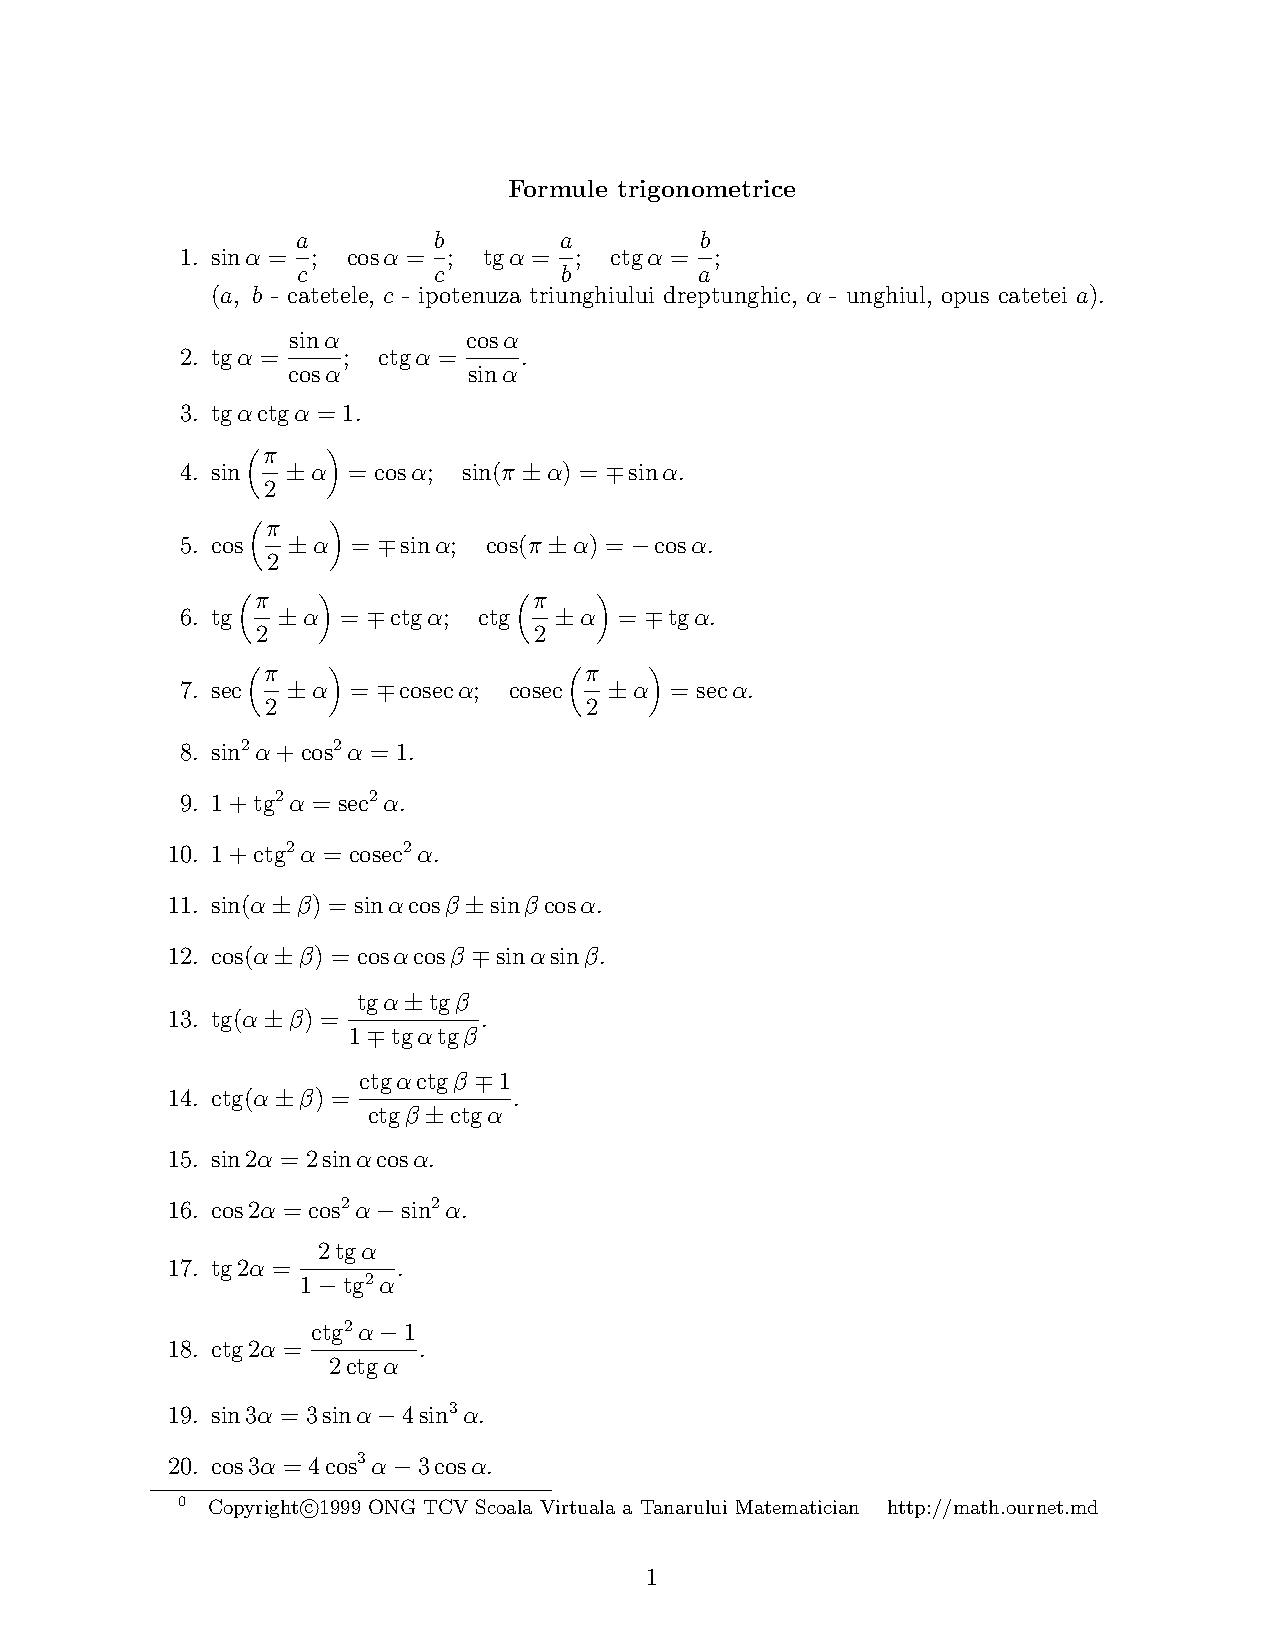
\includepdf[pages=-]{trigonom.pdf}

\chapter[Anexa 3 - Tabele statistice]{Anexa 3 - Tabele statistice}
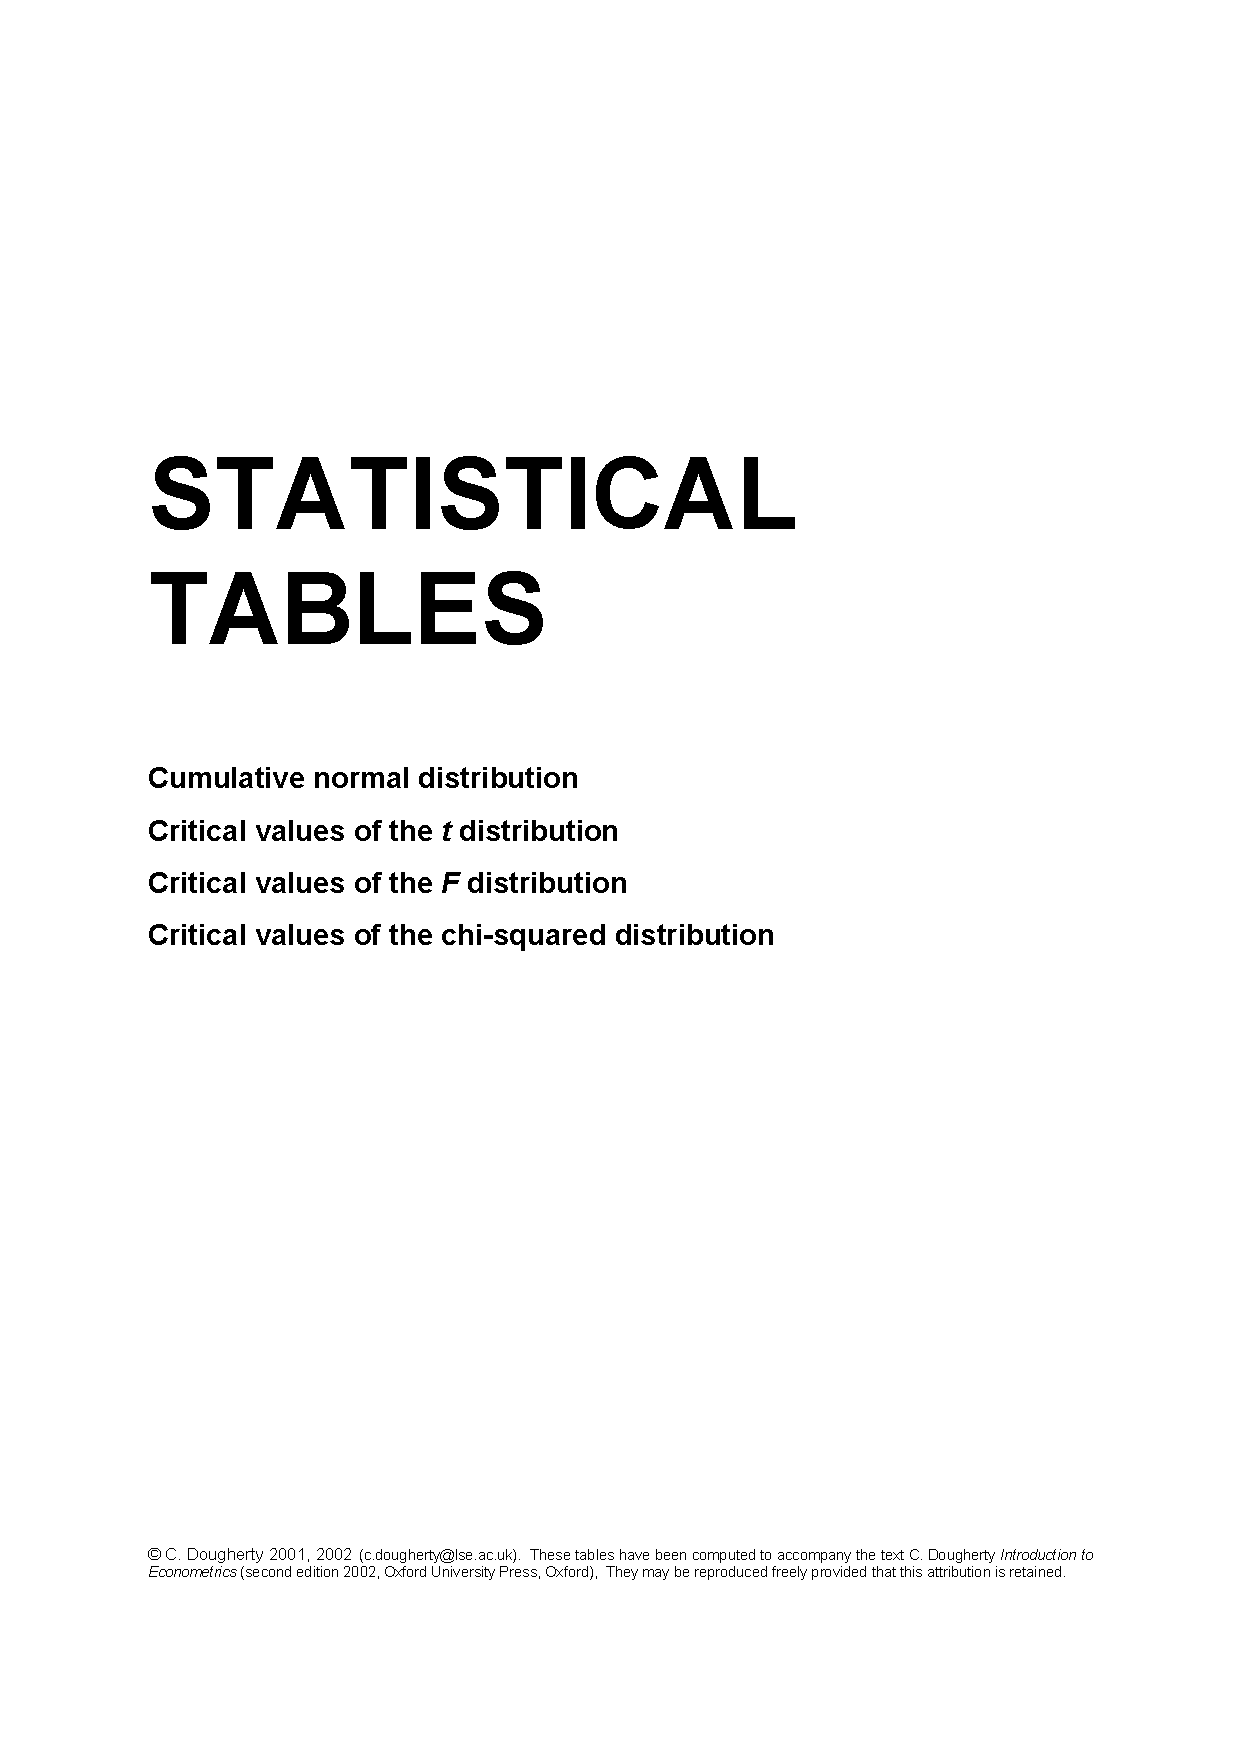
\includepdf[pages=-]{StatistialTables.pdf}



\end{document}